\documentclass[10pt,a4paper]{book}


\usepackage{ctex} 
\usepackage{booktabs}
\usepackage{float}
\usepackage{geometry,graphicx,xcolor,color}
\usepackage{amssymb,amsmath,amsthm}                             % 数学字体
\usepackage{newpxtext,mathpazo}                                % 采用 Palatino 风格字体
\usepackage{newclude,ulem}
\definecolor{winered}{rgb}{0.5,0,0}
\definecolor{structurecolor}{RGB}{122,122,142}
\definecolor{main}{rgb}{0.5,0,0}
\definecolor{second}{RGB}{115,45,2}
\definecolor{third}{RGB}{0,80,80}
\usepackage[colorlinks,linkcolor = winered]{hyperref}           % 定义引用的颜色


% ------------------------------------------------------------%
% 定义定理环境
\usepackage{amsthm}
\newtheoremstyle{defstyle}{3pt}{3pt}{\kaishu}{-3pt}{
	\bfseries\color{main}}{}{0.5em}{\indent 【\thmname{#1} \thmnumber{#2}】 \thmnote{(#3)}}
\newtheoremstyle{thmstyle}{3pt}{3pt}{\kaishu}{-3pt}{
	\bfseries\color{second}}{}{0.5em}{\indent【\thmname{#1} \thmnumber{#2}】 \thmnote{(#3)}}
\newtheoremstyle{prostyle}{3pt}{3pt}{\kaishu}{-3pt}{
	\bfseries\color{third}}{}{0.5em}{\indent【\thmname{#1} \thmnumber{#2}】 \thmnote{(#3)}}

\theoremstyle{thmstyle} %theorem style
\newtheorem{theorem}{定理}[chapter]
\theoremstyle{defstyle} % definition style
\newtheorem{definition}[theorem]{定义}
\newtheorem{lemma}[theorem]{引理}
\newtheorem{corollary}[theorem]{推论}
\theoremstyle{prostyle} % proposition style
\newtheorem{proposition}[theorem]{命题}
\newtheorem{example}[theorem]{例题}

\renewenvironment{proof}[1][证明]{\par{\kaishu \uline{\textbf{#1.}}} \;\fangsong}{\qed\par}
\newenvironment{solution}{\par\underline{\textbf{解.}} \;\kaishu}{\par}
\newenvironment{remark}{\par\underline{\textbf{注.}} \;\fangsong}{\par}
\newcommand{\intro}[1]{\rightline{\parbox[t]{5cm}{\footnotesize \fangsong\quad\quad #1 }}}
% ------------------------------------------------------------%

\usepackage{enumerate}
\usepackage{enumitem}
\setlist[enumerate,1]{label=\color{structurecolor}\arabic*.}
\setlist[enumerate,2]{label=\color{structurecolor}(\arabic*).}
\setlist[enumerate,3]{label=\color{structurecolor}\Roman*.}
\setlist[enumerate,4]{label=\color{structurecolor}\Alph*.}


% 设置章形式
% ---------------------------------- %
% \setlength{\parindent}{0pt}  	
\usepackage{titlesec, titletoc}
\linespread{1.2} 				

\usepackage{fancyhdr}
\fancypagestyle{plain}{%
	\fancyhf{} % clear all header and footer fields
	\renewcommand{\headrulewidth}{0pt}
	\renewcommand{\footrulewidth}{0pt}
}

\titlecontents{chapter}[0em]{}{\large \fangsong{第 \thecontentslabel 章\quad}}{}{\hfill\contentspage}
\titlecontents{section}[2em]{}{\thecontentslabel\quad\textcolor{blue}}{}{\titlerule*{ .} \contentspage}

\titleformat{\chapter}[display]{\Large}
{\color{structurecolor}\centering\small \color{structurecolor}第 \zhnumber{\arabic{chapter}} \ 章 }{0.5ex}
{\color{structurecolor}{\titlerule[1pt]}\Large \kaishu \centering \bfseries}

\titleformat{\section}[frame]
{\normalfont\color{structurecolor}}
{\footnotesize \enspace \large \textcolor{structurecolor}{\S \,\thesection}\enspace}{6pt}
{\Large\filcenter \bf \kaishu }

\titlespacing*{\section}{1pc}{*7}{*2.3}[1pc]
\titleformat{\subsection}[hang]{\bfseries}{
	\large\bfseries\color{structurecolor}\thesubsection\enspace}{1pt}{%
	\color{structurecolor}\large\bfseries\filright}
\titleformat{\subsubsection}[hang]{\bfseries}{
	\large\bfseries\color{structurecolor}\thesubsubsection\enspace}{1pt}{%
	\color{structurecolor}\large\bfseries\filright}

\usepackage{tcolorbox}

% 定义宏包专用的美化框
\newtcolorbox{packagebox}[1]{
	enhanced,
	colback=orange!5!white,
	colframe=orange!75!black,
	fonttitle=\bfseries\large,
	title=#1,
	attach boxed title to top left={yshift=-2mm, xshift=5mm},
	boxed title style={colback=orange!75!black},
	sharp corners=downhill,
	breakable
}
\newtcolorbox{welcomebox}[1]{
	enhanced,
	colback=green!5!white,
	colframe=green!40!black,
	fonttitle=\bfseries\Large,
	title=#1,
	center title,
	drop shadow, % 添加阴影效果
	sharp corners=anticlockwise
}
\newtcolorbox{guwelcome}{
	enhanced,
	boxrule=2pt,
	colback=white,
	colframe=NavyBlue,
	arc=10pt,
	fonttitle=\bfseries\Large,
	title=Hello, Gu!,
	center title,
	attach boxed title to top center={yshift=-3mm},
	boxed title style={colback=NavyBlue},
	drop fuzzy shadow,
	after upper={\par\hfill\textit{--- Welcome to the \LaTeX{} World}}
}
% 定义一个美化版的 colorbox 样式
\newtcolorbox{mybox}[1]{
	colback=blue!5!white,    % 背景色
	colframe=blue!75!black,  % 边框色
	fonttitle=\bfseries,     % 标题字体
	title=#1,                % 标题内容内容
	arc=4pt,                 % 圆角
	outer arc=4pt
}
\usepackage{listings}

\definecolor{codegreen}{rgb}{0,0.6,0}
\definecolor{codegray}{rgb}{0.5,0.5,0.5}
\definecolor{codepurple}{rgb}{0.58,0,0.82}
\definecolor{backcolour}{rgb}{0.95,0.95,0.92}


% 代码块样式全面升级
\lstset{
	language=[LaTeX]TeX,
	basicstyle=\ttfamily\small,
	keywordstyle=\color{blue},
	commentstyle=\color{gray},
	frame=shadowbox,               % 带阴影的边框，更有质感
	rulesepcolor=\color{red!20!green!20!blue!20},
	breaklines=true,
	extendedchars=false            % 解决 listings 处理中文可能出现的乱码问题
}
% --- 设置字体 (请确保你的系统安装了这些字体，或更换为常用字体) ---
\setCJKmainfont{SimSun} % 宋体
\setCJKsansfont{SimHei} % 黑体

% --- 自定义颜色 ---
\definecolor{DarkBlue}{HTML}{1A2B3C}



\begin{document}
	
	% ======================================================
	%                         封面页
	% ======================================================
	\begin{titlepage}
		\begin{tikzpicture}[remember picture, overlay]
			% 1. 背景颜色（可选）
			\fill[white] (current page.south west) rectangle (current page.north east);
			
			\node[anchor=north] at (current page.north) {
				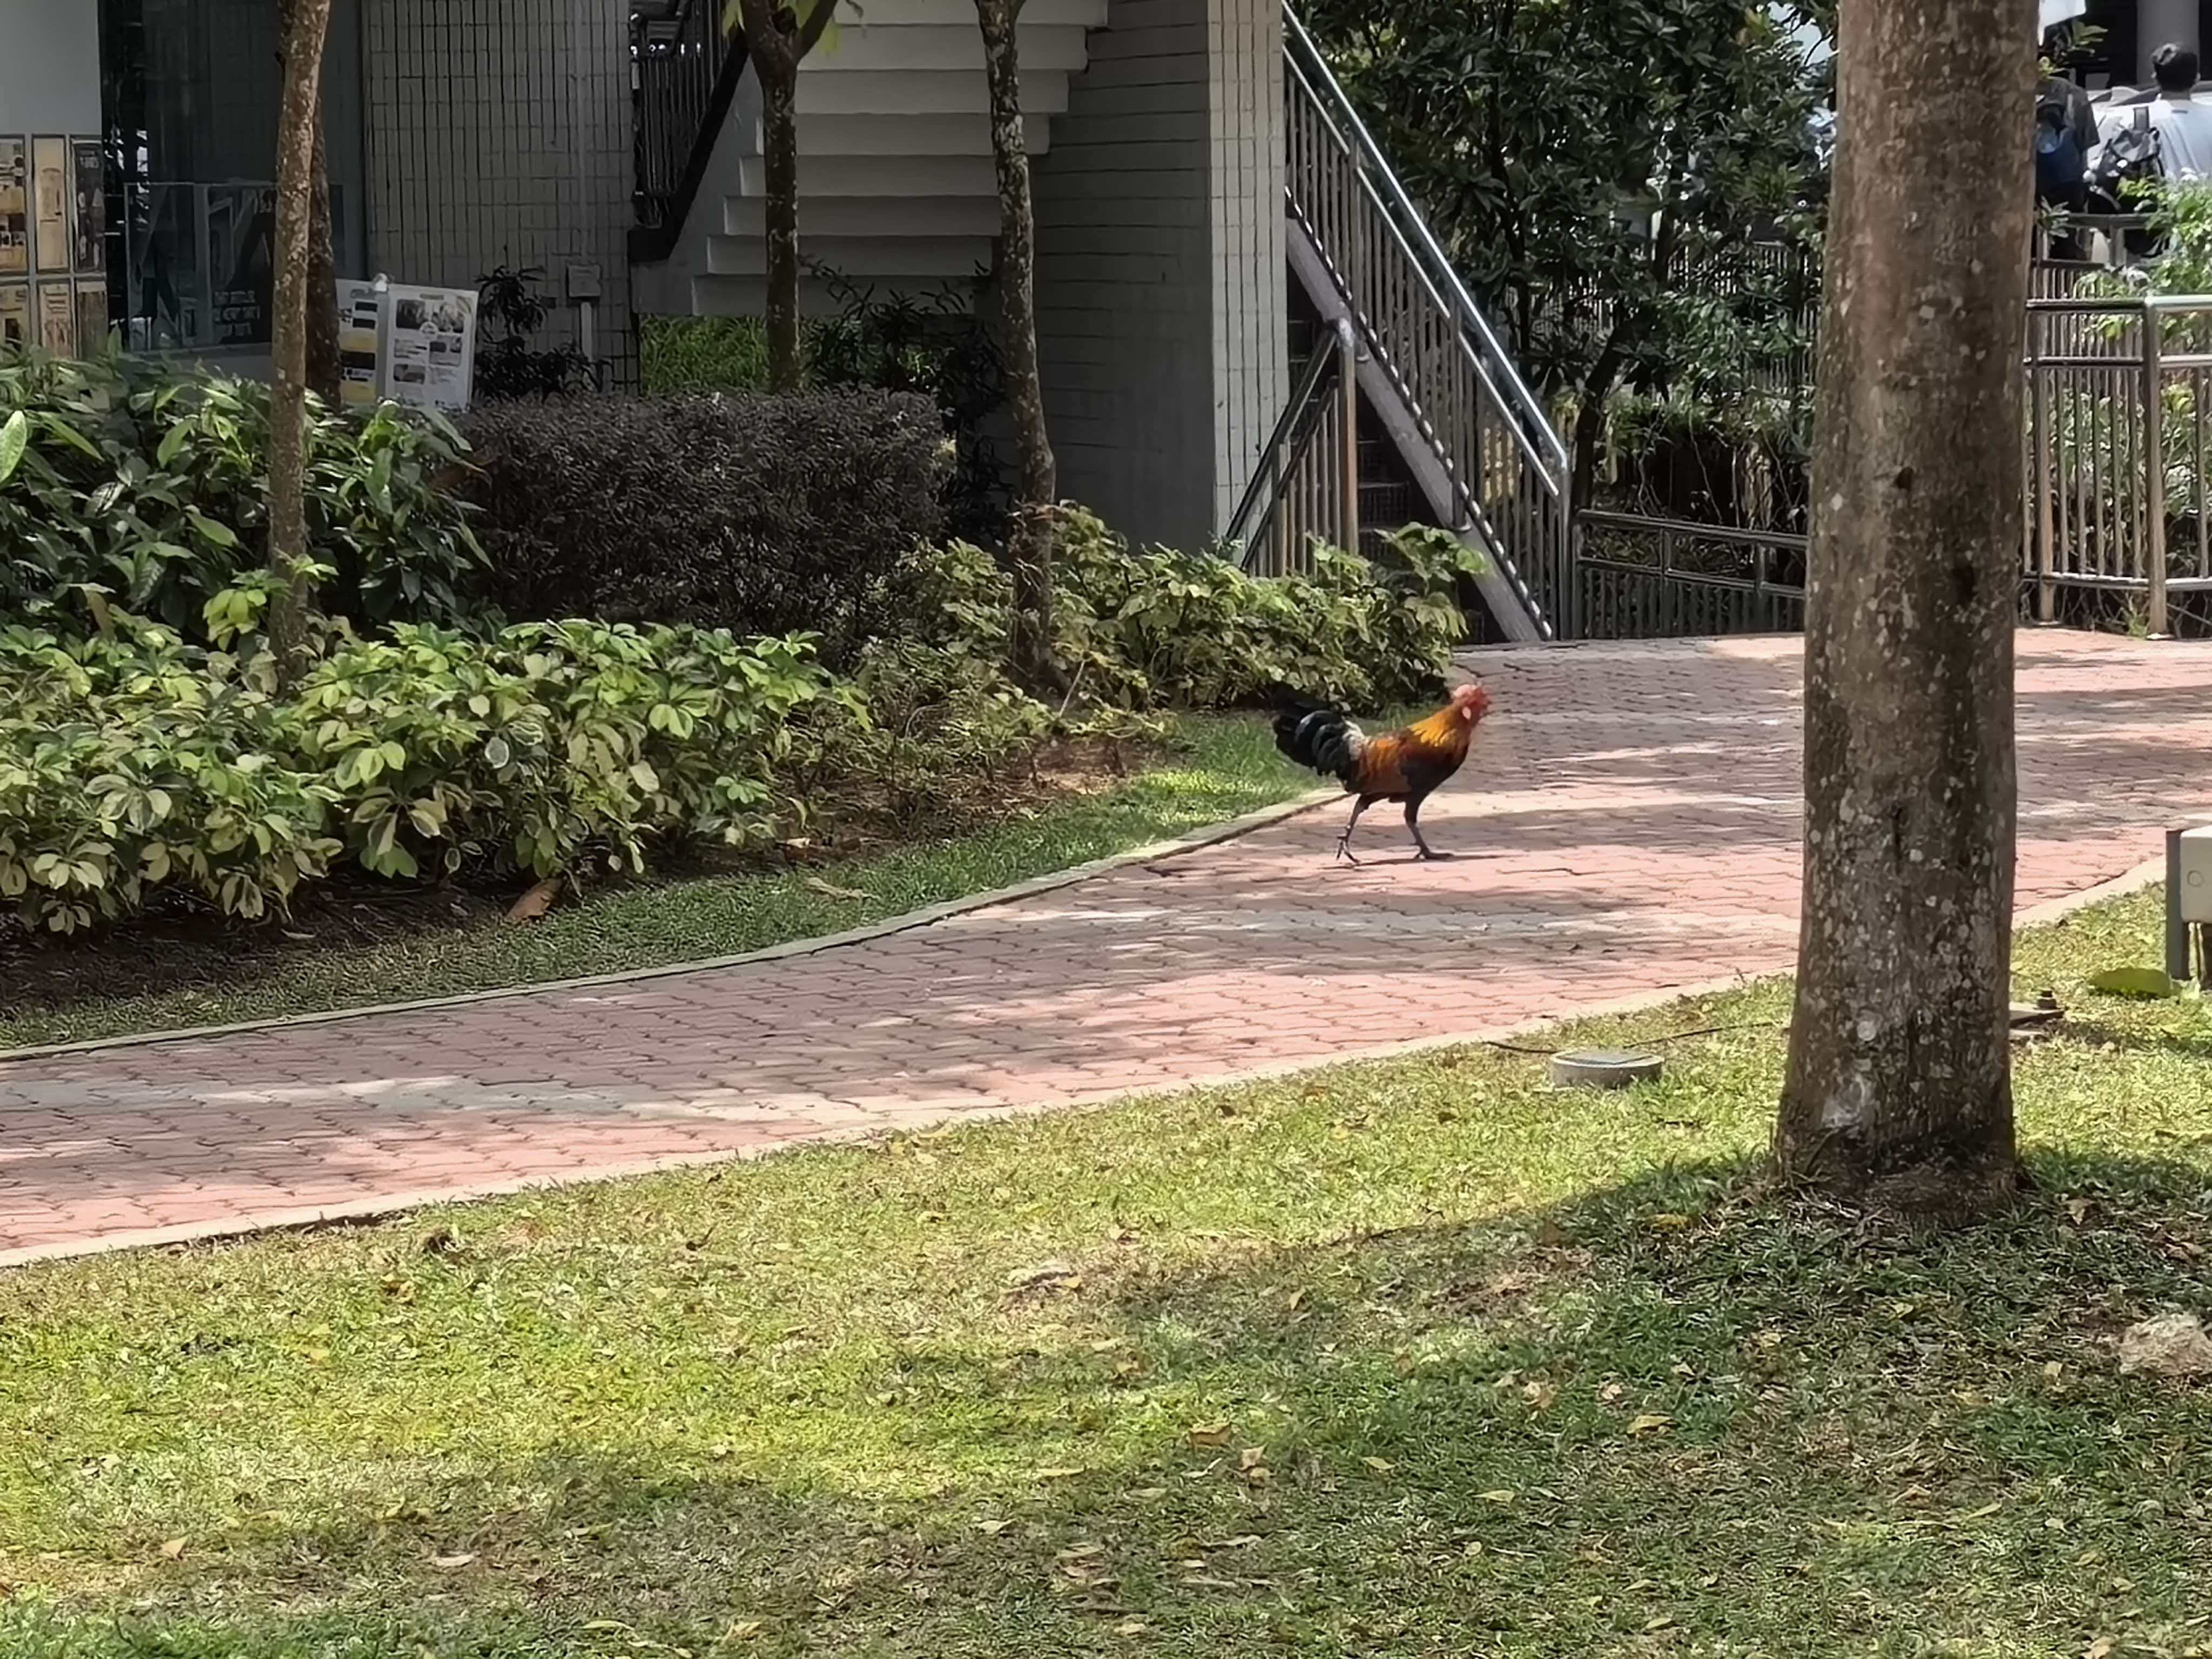
\includegraphics[width=\paperwidth]{d84ddf4a23243a2f0ddf807d2046caed.jpg}
			};
			
			% 3. 装饰条
			\fill[DarkBlue] ([yshift=-12cm]current page.north west) rectangle ([yshift=-12.2cm]current page.north east);
			
			% 4. 标题与作者信息
			\node[anchor=center, text=DarkBlue] at ([yshift=-20cm]current page.north) {
				\begin{minipage}{0.8\paperwidth}
					\centering
					{\fontsize{40}{48}\sffamily\bfseries Markdown小记} \\[1cm]
					{\fontsize{18}{22}\Large 魏舟 \ 著} \\[0.5cm]
					{\large \today}
				\end{minipage}
			};
		\end{tikzpicture}
	\end{titlepage}
	胡翼飞同志问我Markdown怎么用，故写此篇。
	% ======================================================
	%                         目录与正文
	% ======================================================
	\frontmatter
	\tableofcontents
	
	\mainmatter
	\chapter{Markdown编辑器一览}
	\section{Obsidian}
	用过的都说好！因为实时编译，相当于Word的所见即所得。而且支持\LaTeX 的公式语法！（沪爷狂喜）
	自带的插件丰富！便于创建知识点之间的联系！
	所以我一般记笔记选择使用Obsidian。
	\begin{figure}
		\centering
		
\includegraphics[width=0.3\linewidth]{下载}
		\caption{Obsidian图标}
	\end{figure}
	
	而且Obsidian它免费！免费！免费！
	下面是下载网站
	\begin{mybox}{Obsidian下载网址}
		https://obsidian.md/
	\end{mybox}
	下载完不用配置直接使用。
	
	\section{VS code}
	VS code 原生支持Markdown。当然，我们可以下载一些插件使得使用体验更丰富。
	\begin{mybox}{Markdown All in One}
			下面是配置
			\begin{lstlisting}
{
	"markdown.occurrencesHighlight.enabled": true,
	"markdown.preview.fontSize": 16,
	"markdown.preview.linkify": true,
	"markdown.preview.markEditorSelection": true,
	"markdown.preview.openMarkdownLinks": "inEditor",
	"markdown.preview.scrollPreviewWithEditor": true,
	"markdown.updateLinksOnFileMove.enabled": "always",
	"markdown.validate.duplicateLinkDefinitions.enabled": "warning",
	"markdown.validate.enabled": true,
	"markdown.extension.completion.enabled": true,
	"markdown.extension.italic.indicator": "*",
	"markdown.extension.tableFormatter.delimiterRowNoPadding": true,
	"markdown.extension.tableFormatter.normalizeIndentation": true,
	"markdown.extension.theming.decoration.renderLink": true,
	"markdown.extension.theming.decoration.renderParagraph": true,
	"markdown.extension.toc.levels": "2..4",
}
			\end{lstlisting}
	\end{mybox}
	
	
	% --- Markdown 核心语法章节 ---
	\chapter{Markdown 核心语法}
	Markdown 是一种轻量级标记语言，旨在通过纯文本格式实现快速排版。其核心理念是“易读易写”，使用简单的符号来代替复杂的 HTML 标签。
	\section{标题}
	\begin{lstlisting}
# 一级标题
## 二级标题
### 三级标题
#### 四级标题
##### 五级标题
###### 六级标题
	\end{lstlisting}
注：注意井号与标题内容间要空格。
	
	\section{表格}
	使用|来分隔不同的单元格，使用-来分隔表头和其他行：
	\begin{lstlisting}
名字|年龄
---|---
张三|13
	\end{lstlisting}
	
	\section{代码}
	\subsection{代码块}
	代码块中的文本都会显示为原始内容
	\begin{lstlisting}
```语言名称（也可以不指定）
...
	\end{lstlisting}
	\subsection{行内代码}
	也可以通过反引号（``），插入行内代码
	
	\begin{lstlisting}
例 `Markdown`
	\end{lstlisting}
	
	\section{插入图片}
	直接拖就行
	拖进去会自动补全基础语法
	|后面是图片大小
	\begin{lstlisting}
![Alt text|300](图片链接 "optional title")
	\end{lstlisting}
	
	\section{数学公式}
	行内公式： 使用\$包裹公式
	
	独立公式： 使用\$\$包裹公式
	其他语法和 \LaTeX 相同
	\section{总结}
	Markdown 适合快速记录和互联网传播，而 \LaTeX{} 则是出版级论文和复杂学术文档的首选工具。
	
	\begin{mybox}
		
		\Huge 如果你使用Obsidian，上面的都不用学。
		
	\end{mybox}

\end{document}